% tikz_octant.tex -- fig:fundamental-domain, the triangle of deviation directions
% and the regions of the first arc.
%   (a) The sphere of deviation directions, orthogonal to u_0, in orthographic
%       projection along v_1 + w_1 + v_2.  The fundamental triangle of
%       lem:two-symmetries-new is the octant with vertices v_1, w_1, v_2; the
%       faint great circles are the planes of the frame, whose octants are its
%       images under the stabiliser of u_0.  The dashed arcs are the mirrors of
%       the three reflections of the S_3 of lem:s3-symmetry: S (fixes v_1,
%       exchanges w_1, v_2), H (fixes v_2, exchanges v_1, w_1) and SHS (fixes
%       w_1, exchanges v_1, v_2).  They meet at the centroid, fixed by S_3.  The
%       darker small triangle v_1, (v_1+w_1)/sqrt2, centroid is one of the six
%       images; the thick halves of the first two edges are the ranges
%       s in [0, pi/4] of the two arcs.
%   (b) The first arc in the (s, phi) plane, in degrees, to scale: the curves
%       phi = 60 (universal), W: sin s = tan(phi/2), A: cos s = tan(phi/2),
%       Y: sin phi (sin s + cos s) = 1 of thm:arc1-breakpoints-new, crossing at
%       s_1 = arcsin sqrt(2/3) - pi/4 (Y and the universal line, phi = 60),
%       s_2 = arctan(1/2) (W and Y, phi = 48.19 degrees) and
%       s_3 = arcsin(1/sqrt3) (W and the universal line, phi = 60).  The eight
%       regions are shaded by the certificate of thm:arc1-certs-new: exact on
%       region top and on the part 4a of region 4 below W, box covering on
%       the rest.
% Test:   python3 tikz_overlap_check.py tikz_octant.tex
% Build:  pdflatex tikz_octant.tex && pdftoppm -r 500 -png -singlefile tikz_octant.pdf ../figures/fig_tikz_octant
\documentclass[border=4pt]{standalone}
\usepackage{tikz}
\usetikzlibrary{calc,arrows.meta}
\usepackage{pgfplots}
\usepgfplotslibrary{fillbetween}
\pgfplotsset{compat=1.17}
\usepackage[T1]{fontenc}
\usepackage{lmodern}
\usepackage{amsmath,amssymb}
\definecolor{cblue}{HTML}{2A78D6}
\definecolor{corange}{HTML}{EB6834}
\definecolor{caqua}{HTML}{1BAF7A}
\definecolor{cink}{HTML}{0B0B0B}
\definecolor{cink2}{HTML}{52514E}
\definecolor{cink3}{HTML}{8B8A85}
\definecolor{cpanel}{HTML}{F4F3EF}
% tikzcheck.tex -- the hooks of tikz_overlap_check.py, input by the TikZ figures.
% Two ways to name what is checked.
%  - Explicit: \figboxes and \figlabels list named nodes; with \nolabels defined,
%    nodes in the style lbl are drawn invisibly.
%  - Automatic: \autocheck in the preamble gives every node of the picture,
%    pgfplots tick labels included, an alias chk<n>; with \nolabels defined, the
%    text of every node is drawn invisibly and its shape is kept.
% \checkfigure, at the end of the picture, writes the four corners of each
% checked node (so that rotated nodes are measured by their true extent) and
% those of the picture to the log when \checkbboxes is defined.
\tikzset{lbl/.style={}}
\ifdefined\nolabels\tikzset{lbl/.append style={opacity=0}}\fi
\newcount\chknodes
\newcommand\autocheck{% idempotent: a figure with \autocheck may also be run with --auto
  \ifdefined\chkauto\else
  \def\chkauto{}%
  \tikzset{every node/.append style={/utils/exec={\global\advance\chknodes by 1\relax},
                                      alias=chk\the\chknodes}}%
  \ifdefined\nolabels\tikzset{every node/.append style={text opacity=0}}\fi
  \fi}
\makeatletter
% a node counted but never kept (pgfplots typesets some nodes once to measure them)
% has no shape, and is skipped
\newcommand\chkifnode[2]{\pgfutil@ifundefined{pgf@sh@ns@#1}{}{#2}}
\makeatother
\newcommand\chkout[2]{% kind, node
  \path let \p1=(#2.south west), \p2=(#2.north east), \p3=(#2.north west), \p4=(#2.south east)
    in \pgfextra{\typeout{BBOX #1 #2\space\x1\space\y1\space\x2\space\y2\space\x3\space\y3\space\x4\space\y4}};}
\newcommand\checkfigure{%
  \ifdefined\checkbboxes
    \path let \p1=(current bounding box.south west), \p2=(current bounding box.north east)
      in \pgfextra{\typeout{PICBB \x1\space\y1\space\x2\space\y2}};
    \typeout{BORDER 4.0pt}%
    \ifdefined\chkauto
      \edef\chklast{\the\chknodes}%
      \foreach \nm in {1,...,\chklast} {\chkifnode{chk\nm}{\chkout{auto}{chk\nm}}}%
    \else
      \foreach \nm in \figboxes {\chkout{box}{\nm}}%
      \foreach \nm in \figlabels {\chkout{label}{\nm}}%
    \fi
  \fi}
\ifdefined\forceauto\autocheck\fi

\autocheck
% the region shades of (b)
\colorlet{cexact}{caqua!38}
\colorlet{cbox}{cblue!16}
\begin{document}
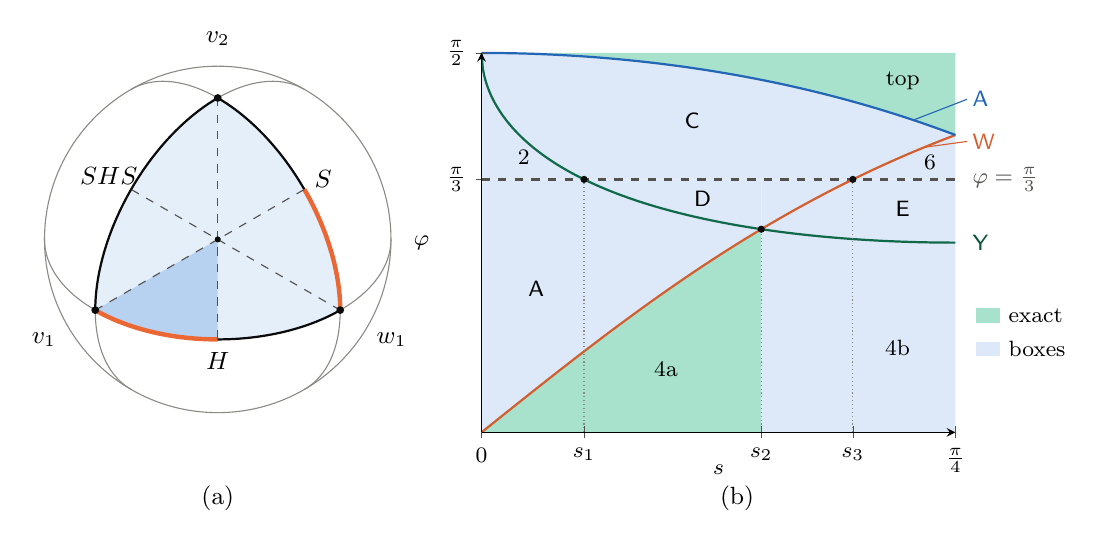
\begin{tikzpicture}[font=\small]
%% ------------------------------------------------------------------ (a)
%% orthographic projection along (1,1,1) in the frame (v_1, w_1, v_2)
\begin{scope}[x={(-1.5556cm,-0.8981cm)}, y={(1.5556cm,-0.8981cm)}, z={(0cm,1.7963cm)}]
  % the limb: the unit circle of the screen, radius 2.2cm
  \draw[cink3, thin] (0,0,0) circle[radius=2.2cm];
  % the fundamental triangle
  \fill[cblue!12] plot[domain=0:90, samples=46, variable=\t] ({cos(\t)},{sin(\t)},0)
     -- plot[domain=0:90, samples=46, variable=\t] (0,{cos(\t)},{sin(\t)})
     -- plot[domain=90:0, samples=46, variable=\t] ({cos(\t)},0,{sin(\t)}) -- cycle;
  % one of the six images under S_3: v_1, (v_1+w_1)/sqrt2, the centroid
  \fill[cblue!34] plot[domain=0:45, samples=24, variable=\t] ({cos(\t)},{sin(\t)},0)
     -- plot[domain=0:54.7356, samples=24, variable=\t] ({0.70711*cos(\t)},{0.70711*cos(\t)},{sin(\t)})
     -- plot[domain=54.7356:0, samples=24, variable=\t] ({cos(\t)},{0.70711*sin(\t)},{0.70711*sin(\t)}) -- cycle;
  % the planes of the frame: front halves faint, back halves not drawn
  \draw[cink3, thin] plot[domain=-45:135, samples=91, variable=\t] ({cos(\t)},{sin(\t)},0);
  \draw[cink3, thin] plot[domain=-45:135, samples=91, variable=\t] (0,{cos(\t)},{sin(\t)});
  \draw[cink3, thin] plot[domain=-45:135, samples=91, variable=\t] ({cos(\t)},0,{sin(\t)});
  % the edges of the triangle
  \draw[cink, thick] plot[domain=0:90, samples=46, variable=\t] ({cos(\t)},{sin(\t)},0);
  \draw[cink, thick] plot[domain=0:90, samples=46, variable=\t] (0,{cos(\t)},{sin(\t)});
  \draw[cink, thick] plot[domain=0:90, samples=46, variable=\t] ({cos(\t)},0,{sin(\t)});
  % the ranges s in [0, pi/4] of the first two arcs
  \draw[corange, line width=1.6pt] plot[domain=0:45, samples=24, variable=\t] ({cos(\t)},{sin(\t)},0);
  \draw[corange, line width=1.6pt] plot[domain=0:45, samples=24, variable=\t] (0,{cos(\t)},{sin(\t)});
  % the three mirrors, each from a vertex to the midpoint of the opposite edge
  \draw[cink2, dashed] plot[domain=0:90, samples=46, variable=\t] ({cos(\t)},{0.70711*sin(\t)},{0.70711*sin(\t)});
  \draw[cink2, dashed] plot[domain=0:90, samples=46, variable=\t] ({0.70711*sin(\t)},{0.70711*sin(\t)},{cos(\t)});
  \draw[cink2, dashed] plot[domain=0:90, samples=46, variable=\t] ({0.70711*sin(\t)},{cos(\t)},{0.70711*sin(\t)});
  % vertices and the centroid
  \fill[cink] (1,0,0) circle (1.4pt);
  \fill[cink] (0,1,0) circle (1.4pt);
  \fill[cink] (0,0,1) circle (1.4pt);
  \fill[cink] (0.57735,0.57735,0.57735) circle (1.1pt);
  % labels: vertices outward, mirrors outside the midpoints of the edges they meet
  \node[inner sep=1.5pt] at (1.42,0,0) {$v_1$};
  \node[inner sep=1.5pt] at (0,1.42,0) {$w_1$};
  \node[inner sep=1.5pt] at (0,0,1.42) {$v_2$};
  \node[inner sep=1.2pt] at (0,0.86,0.86) {$S$};
  \node[inner sep=1.2pt] at (0.86,0.86,0) {$H$};
  \node[inner sep=1.2pt] at (0.89,0,0.89) {$SHS$};
\end{scope}
%% ------------------------------------------------------------------ (b)
\begin{axis}[name=P, at={(3.35cm,-2.45cm)}, anchor=south west, width=7.6cm, height=6.4cm,
    xmin=0, xmax=45, ymin=0, ymax=90,
    axis lines=left, axis on top, tick style={cink2}, tick label style={font=\footnotesize},
    xtick={0,9.7356,26.5651,35.2644,45},
    xticklabels={$0$,$s_1$,$s_2$,$s_3$,$\tfrac\pi4$},
    ytick={60,90},
    yticklabels={$\tfrac\pi3$,$\tfrac\pi2$},
    xlabel={$s$}, ylabel={$\varphi$},
    xlabel style={font=\footnotesize, at={(axis description cs:0.5,-0.06)}},
    ylabel style={font=\footnotesize, rotate=-90, at={(axis description cs:-0.09,0.5)}},
    clip=false]
  \addplot[name path=B0, draw=none, domain=0:45, samples=2] {0};
  \addplot[name path=T, draw=none, domain=0:45, samples=2] {90};
  \addplot[name path=U, draw=none, domain=0:45, samples=2] {60};
  \addplot[name path=W, draw=none, domain=0:45, samples=181] {2*atan(sin(x))};
  \addplot[name path=A, draw=none, domain=0:45, samples=181] {2*atan(cos(x))};
  \addplot[name path=Y, draw=none, domain=0:45, samples=361] {asin(min(1,1/(sin(x)+cos(x))))};
  % exact certificates: region top, and 4a below W
  \addplot[cexact] fill between[of=A and T];
  \addplot[cexact] fill between[of=B0 and W, soft clip={domain=0:26.5651}];
  % box coverings: 4b, A, 2, D, E, 6, C
  \addplot[cbox] fill between[of=B0 and Y, soft clip={domain=26.5651:45}];
  \addplot[cbox] fill between[of=W and U, soft clip={domain=0:9.7356}];
  \addplot[cbox] fill between[of=W and Y, soft clip={domain=9.7356:26.5651}];
  \addplot[cbox] fill between[of=U and Y, soft clip={domain=0:9.7356}];
  \addplot[cbox] fill between[of=Y and U, soft clip={domain=9.7356:26.5651}];
  \addplot[cbox] fill between[of=W and U, soft clip={domain=26.5651:35.2644}];
  \addplot[cbox] fill between[of=Y and W, soft clip={domain=26.5651:35.2644}];
  \addplot[cbox] fill between[of=Y and U, soft clip={domain=35.2644:45}];
  \addplot[cbox] fill between[of=U and W, soft clip={domain=35.2644:45}];
  \addplot[cbox] fill between[of=Y and A, soft clip={domain=0:9.7356}];
  \addplot[cbox] fill between[of=U and A, soft clip={domain=9.7356:35.2644}];
  \addplot[cbox] fill between[of=W and A, soft clip={domain=35.2644:45}];
  % the four curves
  \addplot[cink2, thick, dashed, domain=0:45, samples=2] {60};
  \addplot[corange!90!black, thick, domain=0:45, samples=181] {2*atan(sin(x))};
  \addplot[cblue!85!black, thick, domain=0:45, samples=181] {2*atan(cos(x))};
  \addplot[caqua!60!black, thick, domain=0:45, samples=361] {asin(min(1,1/(sin(x)+cos(x))))};
  % the crossings
  \addplot[cink3, densely dotted] coordinates {(9.7356,0) (9.7356,60)};
  \addplot[cink3, densely dotted] coordinates {(26.5651,0) (26.5651,48.1897)};
  \addplot[cink3, densely dotted] coordinates {(35.2644,0) (35.2644,60)};
  \fill[cink] (axis cs:9.7356,60) circle (1.3pt);
  \fill[cink] (axis cs:26.5651,48.1897) circle (1.3pt);
  \fill[cink] (axis cs:35.2644,60) circle (1.3pt);
  % region names
  \node[inner sep=1pt, font=\footnotesize] at (axis cs:40,83.3) {top};
  \node[inner sep=1pt, font=\footnotesize] at (axis cs:20,74) {$\mathsf C$};
  \node[inner sep=1pt, font=\footnotesize] at (axis cs:4,65.3) {$2$};
  \node[inner sep=1pt, font=\footnotesize] at (axis cs:5.2,34) {$\mathsf A$};
  \node[inner sep=1pt, font=\footnotesize] at (axis cs:17.5,15) {$4$a};
  \node[inner sep=1pt, font=\footnotesize] at (axis cs:39.5,20) {$4$b};
  \node[inner sep=1pt, font=\footnotesize] at (axis cs:21,55.4) {$\mathsf D$};
  \node[inner sep=1pt, font=\footnotesize] at (axis cs:40,53) {$\mathsf E$};
  \node[inner sep=1pt, font=\footnotesize] at (axis cs:42.6,64) {$6$};
  % curve names, to the right of the panel
  \node[anchor=west, inner sep=1.5pt, font=\footnotesize, text=cblue!85!black] at (axis cs:46.2,79) {$\mathsf A$};
  \node[anchor=west, inner sep=1.5pt, font=\footnotesize, text=corange!90!black] at (axis cs:46.2,69) {$\mathsf W$};
  \node[anchor=west, inner sep=1.5pt, font=\footnotesize, text=cink2] at (axis cs:46.2,60) {$\varphi=\tfrac\pi3$};
  \node[anchor=west, inner sep=1.5pt, font=\footnotesize, text=caqua!50!black] at (axis cs:46.2,45) {$\mathsf Y$};
  \draw[cblue!85!black, thin] (axis cs:46.1,79) -- (axis cs:41,74.06);
  \draw[corange!90!black, thin] (axis cs:46.1,69) -- (axis cs:42,67.6);
  % key
  \fill[cexact] (axis cs:47,26) rectangle (axis cs:49.2,29.5);
  \node[anchor=west, inner sep=1.5pt, font=\footnotesize] at (axis cs:49.6,27.75) {exact};
  \fill[cbox] (axis cs:47,18) rectangle (axis cs:49.2,21.5);
  \node[anchor=west, inner sep=1.5pt, font=\footnotesize] at (axis cs:49.6,19.75) {boxes};
\end{axis}
\node[anchor=north, inner sep=2pt] at ($(P.outer south)+(0,0.05cm)$) {(b)};
\node[anchor=north, inner sep=2pt] at ($(0,0)!(P.outer south)!(0,1)+(0,0.05cm)$) {(a)};
\checkfigure
\end{tikzpicture}
\end{document}
